\section{Study of a real product}
\label{sec:study-real-product}

% The studied product is an analog regulation function from automotive world
This chapter details a study case of a real \gls{asic} from the automotive field exposed to \gls{esd} during its normal operation.
The studied chip performs high-level functions with a few of them rather critical for the car vehicle.
Tests and analysis are focused on one function in particular, the primary voltage regulation function of the device.
In the final application, it is powered directly by the car's battery, and starts the entire product.
It is also a good opportunity to study the behavior of a complex analog function exposed to electrostatic discharges.
This product was designed at NXP, and complete access to the schematic and layout was made available for this research work.
The product operation, architecture and application are described in section \ref{sec:product-desc}.

% The chip is used in a lighter configuration where a failure could be identified
This chip has a recommended application circuit provided by NXP, and a specification.
They define many requirements to ensure proper operation, such as supply voltage range, current capability, etc.
Among all those requirements is also defined the minimum constraints for external capacitive decoupling and filtering.
Those constraints are not required by the functionality itself, but are needed to ensure good performance against electrical stresses with some decent margin.
In this research study, the amount of external decoupling and filtering has been reduced intentionally.
The objective is to reduce the bill of materials of the complete application and thus to diminish the cost for the equipment manufacturer.
With this lighter configuration, and by running \gls{esd} simulations, it has been possible to discover a functional weakness.
The failure is described in detailed in section \ref{sec:failure-case-study}.

\subsection{Product description}
\label{sec:product-desc}

% What kind of product
An actual automotive \gls{asic} was tested to highlight a practical case of functional failure.
The tested \gls{asic} performs several high-level and critical functions in the car.

% What kind of failure
The failure was discovered while reducing the amount of external devices, to test the impact on the robustness.
With less external devices, the bill of materials of the electronic system is reduced and the system costs less to manufacture.
It must be clarified that with the normal configuration, the failure never happens (within limits of the \gls{esd} tester).
It can only be reproduced in this lowered configuration.

% Difference of configs
The input used during the tests to inject the \gls{ESD} is the battery supply connection.
The normal configuration uses strong differential and common-mode filtering on this input.
This technique very effectively deviates the stress current into a ground before it even has a chance to reach the tested chip.
In the lowered-configuration, only a reduced differential filtering is present on the input.

% What is being tested
Inside the \gls{ic}, the study focuses on the primary supply function.
More specifically, the behavior of a 2.5V internal DC-DC LDO (glossary ?) regulator is under test.
This function is responsible for waking up all other integrated functions, and powers digital cells.
It plays a key part in the device's operation, and constitutes an interesting study case.
Also, this function requires for normal operation a large stabilisation capacitor that cannot be integrated on silicon.
A pin is exposed externally to let the board manufacturer connect such a capacitor at the board level.
This pin makes for a very easy monitoring point during tests, without needing to open the package to measure signals.

% Global architecture
Fig. \ref{fig:system_architecture} details the architecture of a typical system using the chip under test.

\begin{figure}[!htbp]
  \centering
  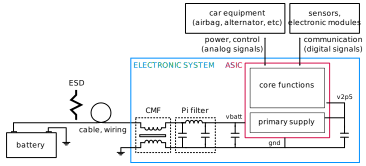
\includegraphics[width=0.9\textwidth]{src/3/figures/architecture_system.pdf}
  \caption{Overview of the system architecture}
  \label{fig:system_architecture}
\end{figure}

GO DOWN INTO ASIC, explain architecture a bit

\begin{figure}[!htbp]
  \centering
  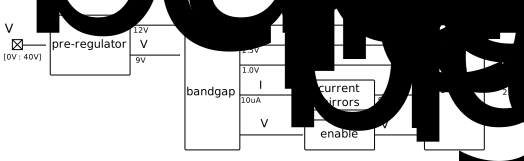
\includegraphics[width=0.9\textwidth]{src/3/figures/monitored_function.pdf}
  \caption{Architecture of the monitored function}
  \label{fig:monitored_function_first}
\end{figure}

SHOW Startup curves ?

\subsection{Functional failure study}
\label{sec:failure-case-study}

% How is the failure produced
A negative \gls{tlp} pulse is injected on top of the \gls{dc} supply, connected to the input pin V\textsubscript{batt}.
The width of the discharge is the usual \SI{100}{\nano\second}, with a risetime of \SI{1}{\nano\second}.
Failures start to appear with pulse amplitudes larger than \SI{-80}{\volt}.
The failure is observed on the V\textsubscript{2p5} output pin (Fig. \ref{fig:meas-reset-v2p5}).
To perform the injection, the battery is replaced by a \gls{dc} source and a \gls{tlp} generator.
Both devices are isolated from one another using a \gls{bias-tee}, as defined in the DPI standard \cite{iec62132-4}.
This setup is simply a capacitor-inductor network as shown in Fig. \ref{fig:injection-setup-dpi}.

\begin{figure}[!h]
  \centering
  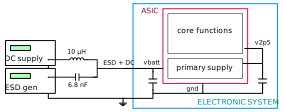
\includegraphics[width=0.7\textwidth]{src/3/figures/architecture_system_test.pdf}
  \caption{Injection setup to superimpose a stress on a DC voltage}
  \label{fig:injection-setup-dpi}
\end{figure}

% What is the root cause -> reset of regulator, soft-start
The failure signature recorded on V\textsubscript{2p5} is given in Fig. \ref{fig:meas-reset-v2p5}.
The area of the curve in red corresponds to the entire restart.
The nominal value for V\textsubscript{2p5} is \SI{2.5}{\volt}.
The \gls{tlp} pulse is visible at \SI{53}{\micro\second}.
After a small delay of about \SI{2}{\micro\second}, the regulation function slowly shuts down.
The output voltage falls for nearly \SI{30}{\micro\second} until reaching a voltage of \SI{1.5}{\volt}.
At this point, the supply cannot reliably power digital gates for instance, and is completely at fault.
Afterwards, a new soft-start sequence begins.
A soft-start normally happens only during system power-up, when the main external supply is switched on.
During a soft-start, the supply voltage slowly rises from \SI{0}{\volt} to its nominal value.
It avoids overshoots that could damage sensitive blocks, and is a slow procedure that takes tens of microseconds to complete.
The shut-down followed by the soft-start lasts in total about \SI{50}{\micro\second}.
It corresponds to the time it takes for the signal V\textsubscript{2p5} to recover.
In comparison, the input disturbance on V\textsubscript{batt} lasts only \SI{100}{\nano\second}.

\begin{figure}[!h]
  \centering
  \includegraphics[width=0.9\textwidth]{src/3/figures/v2p5_measure.png}
  \caption{Measurement of V\textsubscript{2p5} after a \SI{-100}{\volt} \SI{100}{\nano\second} negative stress}
  \label{fig:meas-reset-v2p5}
\end{figure}

% Discuss lack of impact of positive stress
Testing was also conducted using positive stresses, however no failure could be triggered up to the maximum discharge level.
The integrated circuit seems much more sensitive to negative discharges.
After this preliminary testing on a real chip, the analysis is conducted with simulation tools to understand how the failure appears internally.

% Compare sim and meas for Vbatt
A transient simulation of the integrated regulation function is ran.
It uses the transistor-level schematic of the function, and its surrounding environment composed of decoupling capacitors, printed circuit board, \gls{dc} sources and test generator.
The simulation of V\textsubscript{batt} is compared to a measurement in Fig. \ref{fig:wvf-vbatt}.
The simulation setup reproduces the measurement setup, using the modeling approach presented in previous chapter.
During the discharge, V\textsubscript{batt} has a larger amplitude in simulation, and reaches a more negative voltage.
The positive overshoot after the pulse is correctly reproduced, although it dampens slower in the simulation.
It looks like the measurement has less bandwidth than the simulation.
The accuracy is not great, but it is sufficient to reproduce the failure on the output.
Also, the timescale is much shorter in Fig. \ref{fig:wvf-vbatt} than in Fig. \ref{fig:meas-reset-v2p5} and the analysis focuses here on events longer than a few microseconds.

\begin{figure}[!h]
  \centering
  \includegraphics[width=0.95\textwidth]{src/3/figures/vbatt.png}
  \caption{Measurement and simulation for V\textsubscript{batt} (short timescale)}
  \label{fig:wvf-vbatt}
\end{figure}

% Compare sim and meas for V2p5
Fig. \ref{fig:wvf-v2p5} provides the same comparison for V\textsubscript{2p5}.
The reset is clearly visible on both simulation and measurement.
The restart happens almost at the same time in both waveforms, at about \SI{32}{\micro\second} after the stress was injected.
Right after the \gls{esd} injection, the disturbance amplitude is a bit larger in simulation.
But overall, the accuracy is satisfying.
Both comparisons tend to indicate that simulations can be trusted to reproduce the failure in this study case.

\begin{figure}[!h]
  \centering
  \includegraphics[width=0.9\textwidth]{src/3/figures/v2p5.png}
  \caption{Measurement and simulation of the functional failure on V\textsubscript{2p5}}
  \label{fig:wvf-v2p5}
\end{figure}

% Now use the simulation for analysis
So far, the waveforms of V\textsubscript{batt} (external input) and V\textsubscript{2p5} (external output) were shown.
Simulations are now employed to observe the intermediate nets inside the integrated circuit.
The waveform for the internal output V\textsubscript{clamp9} of the pre-regulator is given in Fig. \ref{fig:wvf-vclamp9}.
The timescale is shorter than the previous curves.
At \SI{54}{\micro\second},  V\textsubscript{clamp9} is disturbed by the negative stress, in two phases.
The first phase is \SI{100}{\nano\second} wide, and corresponds to the direct exposure to the stress.
During this phase, V\textsubscript{clamp9} reaches as low as \SI{0}{\volt} for a brief amount of time.
Afterwards, there is a second phase, that lasts approximately \SI{650}{\nano\second}.
This second undervoltage will not be detailed but can be explained by the design and architecture of the block.
Overall, V\textsubscript{clamp9} is disturbed for \SI{750}{\nano\second}.

\begin{figure}[!h]
  \centering
  \includegraphics[width=0.95\textwidth]{src/3/figures/vclamp9.png}
  \caption{Simulated waveform of the V\textsubscript{clamp9} internal net (short timescale)}
  \label{fig:wvf-vclamp9}
\end{figure}

% Next net, bandgap input
V\textsubscript{clamp9} is used as a power supply for the bandgap reference.
The bandgap is expected to be disturbed because of the variation on V\textsubscript{clamp9}.
The observation of the \SI{1.0}{\volt} bandgap reference V\textsubscript{ref1p0} confirms it (Fig. \ref{fig:wvf-v1p0}).
The reference drops down to \SI{0.25}{\volt}, and is disturbed for about \SI{3}{\micro\second}.

\begin{figure}[!h]
  \centering
  \includegraphics[width=0.9\textwidth]{src/3/figures/v1p0.png}
  \caption{Simulated waveform of the V\textsubscript{ref1p0} internal net}
  \label{fig:wvf-v1p0}
\end{figure}

% Final net
Finally, V\textsubscript{ref1p0} is used by the regulator to generate the \SI{2.5}{\volt} external supply output V\textsubscript{2p5}.
Previously,  Fig. \ref{fig:wvf-v2p5} showed that V\textsubscript{2p5} drops below \SI{1.5}{\volt}, and is disturbed for more than \SI{30}{\micro\second}.

% Preliminary conclusion with scale factor
There is a clear trend regarding the duration of the failure.
In the first block (pre-regulator), the disturbance width increased from \SI{100}{\nano\second} to \SI{750}{\nano\second}.
In the second block (bandgap), it increased from \SI{750}{\nano\second} to \SI{3}{\micro\second}.
In the third block (regulator), it reached \SI{30}{\micro\second}.
After each block, there is an aggravation or an amplification of the failure.
Ultimately, the final regulation function that takes a lot of time to recover is hit, causing a full system restart.

% Transition
The next part of this research work is focused on developing measurement methods to acquire data at the silicon level, to confirm the simulations.
A testchip is designed to validate new measurement and observation methods in section \ref{sec:test-vehicle-desc}.
Modeling methods are explored in section \ref{sec:bottom-up-modeling} as a way to understand and predict these functional issues.

